\documentclass[a4paper,12pt]{article}
\usepackage{hyperref}
\usepackage{graphicx}

\begin{document}

\title{Guide for uploading of multiple lectures/assignments}
\author{Tim van der Lippe \& Gijs Weterings}
\maketitle

\newpage

\section{Upload lectures}

To upload multiple lectures at the same time, the format of \url{https://mytimetable.tudelft.nl/} is used.
This guide will describe how to export your lectures from \url{https://mytimetable.tudelft.nl/} into the planningstool.

\begin{enumerate}
  \item Log in to \url{https://mytimetable.tudelft.nl/}

  \item Click on "Export" (Button next to "Add timetable")

  \item Under "Download", click "CSV (Excel)" and save the downloaded file in a convenient location

  \item Log in to the planningstool

  \item Under Assignments "Create", click "Upload lectures" and select the file you downloaded

\end{enumerate}

\section{Upload assignments}

The format for assignments is as follows:

\[CourseId;Year;Length;Title;Description;Weeknumber\]

The Weeknumber is the first upcoming week with this number.
E.g. in week 50 of 2015, WeekNumber 3 corresponds to week 3 in year 2016.
E.g. in week 5 of 2016, WeekNumber 20 corresponds to week 20 in year 2016.

A valid CourseId and Year are those in the Course dropdown under Assignments "Create" in the planningstool.
In the image below, the first CourseId is "TI1505" and the Year is "2015".

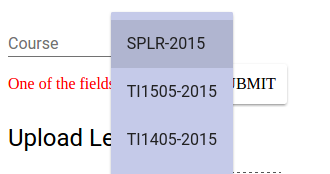
\includegraphics[width=5cm]{courses.png}

\end{document}
